\chapter{GENEL İŞLEMCİ MİMARİSİ}
İşlemci tasarımı buyruk kümesinin tasarlanması ile başlar. Daha sonra buyrukların koşturulabilmesi için gerekli donanımlar belirlenir ve bu donanımların yüksek verimli kullanımını sağlamak için boru hattı mimarisi tasarlanır. Tezin bu bölümünde öncelikli olarak buyruk kümesi mimarisi anlatılacak, ardından her buyruğun ihtiyaç duyduğu hesaplama modülleri belirlenecek, sonrasında kullanım senaryoları üzerinden boru hattı mimarisi tasarımı anlatılacaktır. Son olarak Tosun işlemcisinin veri yolu mimari yapısı ve tasarım kararları üzerinde durulacaktır.\par

\section{Buyruk Kümesi Mimarisi}
Hedeflenen işlemciye benzer özelliklerde mevcut paralel işlemcilerin buyruk kümesi mimarileri incelenmiş, gereksinim analizinde fonksiyonların gerçeklenebilmesi için gerekli olarak belirlenen buyruklar bu buyruk kümesi mimarilerine eklenerek Tosun işlemcisi için bir buyruk kümesi mimarisi oluşturulmuştur. Mevcut buyruk kümelerinin incelenmesinin sebebi paralel işlemcilerin mimari özelliklerinden bağımsız olarak sahip olması gereken ortak özelliklerin bulunmasıdır. Bu özelliklerden bazıları yükleme ve saklama operasyonları, threadler arası senkronizasyonun sağlanması, çekirdeklerin bellek erişimlerinde kullanılan adres hesaplamaları, yazmaçlar üzerinde yapılan okuma ve yazma işlemleridir. \par

Tosun buyruk kümesi mimarisinin oluşturulmasında NVidia PTX \cite{nvidiaPTXISA} buyruk kümesi paralel işleme mimarisi olarak temel alınmıştır. Ayrıca adres hesapları, dallanmalar, temel aritmetik ve mantık işlemleri gibi her işlemcinin sahip olması gereken temel buyruklar için de Intel x86 \cite{x86ISA} ve MIPS \cite{MIPSISA} buyruk kümeleri referans alınmıştır. \par

Tosun buyruk kümesi mimarisinde bulunmasına karar verilen buyruklar tablo \ref{table:tosunInstructions} içinde sunulmuştur. 



\begin{longtable}{p{50pt} p{300pt} p{70pt}}
\caption{Tosun Buyruk Listesi} \label{table:tosunInstructions} \\
\multicolumn{1}{l}{\textbf{Buyruk}} & \multicolumn{1}{l}{\textbf{Açıklama}} & \multicolumn{1}{c}{\textbf{Türü}} \\ 
\hline 
\endfirsthead

\multicolumn{2}{c}%
{{\bfseries \tablename\ \thetable{} -- devam}} \\
\multicolumn{1}{l}{\textbf{Buyruk}} &
\multicolumn{1}{l}{\textbf{Açıklama}} &
\multicolumn{1}{c}{\textbf{Türü}}  \\ \hline 
\endhead

\hline \multicolumn{2}{r}{{Sonraki sayfada devam etmektedir.}} \\ 
\endfoot

\hline \hline
\endlastfoot
  addi		&	 $r_{d} = r_{s1} + 			$anlık 	& \multicolumn{1}{c}{Anlık} 	\\
  andi 		&	 $r_{d} = r_{s1} \& 		$anlık 	& \multicolumn{1}{c}{Anlık}  	\\
  ori 		&	 $r_{d} = r_{s1} | 			$anlık  & \multicolumn{1}{c}{Anlık}  	\\
  xori 		&	 $r_{d} = r_{s1} \oplus $anlık 	& \multicolumn{1}{c}{Anlık}  	\\
  divi 		&	 $r_{d} = r_{s1} / 			$anlık  & \multicolumn{1}{c}{Anlık}  	\\
  muli 		&	 $r_{d} = r_{s1} x 			$anlık  & \multicolumn{1}{c}{Anlık}  	\\
  subi 		&	 $r_{d} = r_{s1} - 			$anlık  & \multicolumn{1}{c}{Anlık}  	\\
  movi 		&	 $r_{d}(alt) = 	$anlık  & \multicolumn{1}{c}{Anlık}  	\\
  movhi		&	 $r_{d}(ust) = 	$anlık  & \multicolumn{1}{c}{Anlık}  	\\
  fabs  	&  $r_{d} = |r_{s1}|			$				&	\multicolumn{1}{c}{Y1}		 	\\
  fadd  	&  $r_{d} = r_{s1} + r_{s2}$			&	\multicolumn{1}{c}{Y2}		 	\\
  fcom  	&  $r_{d} = com(r_{s1},r_{s2})$		&	\multicolumn{1}{c}{Karşılaştırma}	 	\\
  fdiv  	&  $r_{d} = r_{s1} / r_{s2}$			&	\multicolumn{1}{c}{Y2}		 	\\
  fmul  	&  $r_{d} = r_{s1} x r_{s2}$			&	\multicolumn{1}{c}{Y2}		 	\\
  fsqrt  	&  $r_{d} = sqrt(r_{s1})$					&	\multicolumn{1}{c}{Y1}		 	\\
  fcos  	&  $r_{d} = cos(r_{s1})$					&	\multicolumn{1}{c}{Y1}		 	\\
  fsin  	&  $r_{d} = sin(r_{s1})$					&	\multicolumn{1}{c}{Y1}		 	\\
  ffma  	&  $r_{d} = r_{s1}xr_{s2}+r_{s3}$	&	\multicolumn{1}{c}{Y3}		 	\\
  ffms  	&  $r_{d} = r_{s1}xr_{s2}-r_{s3}$	&	\multicolumn{1}{c}{Y3}		 	\\
  fmin  	&  $r_{d} = min(r_{s1},r_{s2})$		&	\multicolumn{1}{c}{Y2}		 	\\
  fmax  	&  $r_{d} = max(r_{s1},r_{s2})$		& \multicolumn{1}{c}{Y2}			\\
  fln 	 	&	 $r_{d} = log_{e}(r_{s1})$			& \multicolumn{1}{c}{Y1}			\\
  fmod 		&	 $r_{d} = r_{s1} \% r_{s2} $ 		& \multicolumn{1}{c}{Y2}  		\\
  f2int 	&	 $r_{d} = r_{s1}$ 							& \multicolumn{1}{c}{Y1}  		\\
  int2f		&	 $r_{d} = r_{s1}$ 							& \multicolumn{1}{c}{Y1}  		\\
  fchs		&	 $r_{d} = -r_{s1}$ 							& \multicolumn{1}{c}{Y1}  		\\
  fexp 		&	 $r_{d} = e^{r_{s1}}$						& \multicolumn{1}{c}{Y1}  		\\
  add 		&	 $r_{d} = r_{s1} + r_{s2}$ 			& \multicolumn{1}{c}{Y2}  		\\
  and 		&	 $r_{d} = r_{s1} \& r_{s2}$ 		& \multicolumn{1}{c}{Y2}  		\\
  or 			&	 $r_{d} = r_{s1} | r_{s2}$			& \multicolumn{1}{c}{Y2}  		\\
  xor			&	 $r_{d} = r_{s1} xor r_{s2}$ 		& \multicolumn{1}{c}{Y2}  		\\
  div  		&  $r_{d}	= r_{s1} / r_{s2}$			&	\multicolumn{1}{c}{Y2}		 	\\
  mul  		&  $r_{d} = r_{s1} x r_{s2}$			&	\multicolumn{1}{c}{Y2}		 	\\
  shl  		&  $r_{d} = r_{s1} << r_{s2}$			&	\multicolumn{1}{c}{Y2}		 	\\
  shr  		&  $r_{d} = r_{s1} >> r_{s2}$			&	\multicolumn{1}{c}{Y2}			\\
  shra  	&  $r_{d} = r_{s1} >> r_{s2}$			&	\multicolumn{1}{c}{Y2}		 	\\
  sub  		&  $r_{d} = r_{s1} - r_{s2}$			&	\multicolumn{1}{c}{Y2}		 	\\
  min  		&  $r_{d} = min(r_{s1},r_{s2})$		&	\multicolumn{1}{c}{Y2}		 	\\
  max  		&  $r_{d} = max(r_{s1},r_{s2})$		&	\multicolumn{1}{c}{Y2}		 	\\
  chs  		&  $r_{d} = -r_{s1}$							&	\multicolumn{1}{c}{Y1}		 	\\
  not  		&  $r_{d} = ~r_{s1}$							&	\multicolumn{1}{c}{Y1}		 	\\
  abs  		&  $r_{d} = |r_{s1}|$							&	\multicolumn{1}{c}{Y1}		 	\\
  com  		&  $r_{d} = max(r_{s1},r_{s2})$		& \multicolumn{1}{c}{Y2}			\\
  mod  		&  $r_{d} = max(r_{s1},r_{s2})$		& \multicolumn{1}{c}{Y2}			\\
  brv 		&	 Verilen yazmaçtaki bitleri ters sırada hedef yazmaca yazar & \multicolumn{1}{c}{Y1}  \\
  bfr 		&	 Verilen yazmacın belirtilen kadar kısmını maskeleyip hedef yazmaca yazar & \multicolumn{1}{c}{Y1}  \\
  br 			&	 Karşılaştırma bayraklarında belirtilen koşul varsa, verilen adres kadar ileri atlar & \multicolumn{1}{c}{Dallanma}  \\
  fin 		&	 Programı sonlandırır& \multicolumn{1}{c}{Sistem}  \\
  ldshr 	&	 Paylaşımlı bellekten yükleme işlemi yapar& \multicolumn{1}{c}{Y1}  \\
  stshr 	&	 Paylaşımlı belleğe saklama işlemi yapar& \multicolumn{1}{c}{Y1}  \\
  sync		&	 Tüm threadler aynı noktaya gelinceye kadar önce gelen threadleri bekletir. & \multicolumn{1}{c}{Sistem}  \\
  ldram 	&	 Ana bellekten yükleme işlemi yapar& \multicolumn{1}{c}{Y1}  \\
  stram		&	 Ana belleğe saklama işlemi yapar& \multicolumn{1}{c}{Y1}  \\
  mov 		&  $r_{d}$ = $r_{s1}$ 						&	\multicolumn{1}{c}{Taşıma}		 \\
  jmp  		&  Program sayacına belirtilen sayıyı ekleyerek atlar &	\multicolumn{1}{c}{Atlama}		 \\
  
\end{longtable}

Tosun buyruk kümesinde toplam 56 adet buyruk belirlenmiştir. Tablo \ref{table:tosunInstructions} içinde verilen buyruklar içerdikleri işlenen tür ve sayılarına göre türlere ayrılmıştır. Bu sınıflandırma buyruk içinde belirtilmesi gereken işlenen cins ve sayılarına göre yapılmıştır. Buyruk türlerinin bit yapısının belirlenebilmesi için öncelikle buyruk içine yerleştirilecek bilgilerin bit genişlikleri belirlenmelidir. \par

Buyruk bit yapılarında kaynak ve hedef hafıza birimleri olarak yazmaç numaraları kullanılır. Buyruk içinde bir yazmacın kaç bit ile ifade edileceği, bir thread için tahsis edilen yazmaç sayısına bağlıdır. İşlemci mimarisinde yazmaç sayısının belirlenmesi bir ödünleşimli karardır. Yazmaç sayısının artması yazmaçlar için kullanılan alanı artıracağı gibi yazmaç numaraları için kullanılan karşılaştırıcı devrelerin de büyümesine sebep olur. Öte yandan yazmaç sayısının azlığı bellek işlemlerinin artmasına ve başarımın düşmesine sebep olacaktır. Tosun mimarisinde çok çekirdekli bir mimariden söz edildiği için yazmaç sayılarının artışı tek çekirdekli işlemcilere oranla daha fazla bir alan kullanımında artışa sebep olmaktadır. Bu yüzden Tosun mimarisinde hedef programlara yetebilecek minimum sayıda yazmaç kullanılmıştır. Bu çalışmada NVidia CUDA ile çalışan 184 adet paralel hesaplama uygulamasının yazmaç kullanım adetleri incelenmiştir. Elde edilen sonuçlara göre Tablo \ref{table:NVidiaRegisterUsage}'ta sunulduğu şekilde 64 adetten fazla sayıda yazmaç kullanan program ile karşılaşılmamıştır.

\begin{longtable}{p{350pt} p{100pt} }
\caption{NVidia GPGPU Programları Yazmaç Kullanım Analizi} \label{table:NVidiaRegisterUsage} \\
\multicolumn{1}{l}{\textbf{Açıklama}} & \multicolumn{1}{r}{\textbf{Adet}}  \\ 
\hline 
\endfirsthead
32 veya daha az sayıda yazmaç kullanan uygulamalar  & \multicolumn{1}{r}{138} \\
32 ile 64 adet arasında yazmaç kullanan uygulamalar & \multicolumn{1}{r}{46}  \\
64 yazmaçtan fazla sayıda yazmaç kullanan uygulamalar & \multicolumn{1}{r}{0} \\
\end{longtable}

Neticede her bir thread için 64 adet yazmaçtan oluşan yazmaç öbeği kullanılmasına karar verilmiştir. Projenin bir diğer isteği olan OpenCL desteği ise OpenCL spesifikasyonlarında belirtilen bazı özel amaçlı yazmaçların gerçeklenmesini zorunlu kılmaktadır. Lokal thread numarası ve global thread numarası gibi programcının erişimine açık olması gereken ve spesifikasyonda belirtilen bilgiler program içinde özellikle adres hesaplamalarında sıklıkla kullanılmakta olduğundan yazmaç öbeğinde tutulması faydalı olacaktır. Bu bilgilerin yanı sıra program parametrelerinin de yazmaç öbeğine dahil edilmesi ile yazmaç sayısı 128 adete çıkarılmıştır. Ancak 128 yazmacın yalnızca ilk 64 adedi genel amaçlı olup, son 64 adeti özel mov buyruğu ile erişilebilir olarak belirlenmiştir. Toplamda 64 adet genel amaçlı yazmaç, buyruk içinde 6 bit ile ifade edilebilir. \par

Tüm işlemler 32 bit genişliğinde float veya tam sayılar ile yapılmaktadır. Yazmaç sayıları ve işlem kodu da hesaba katıldığında genel olarak buyrukların 32 bit genişliğe sığdırılabileceği hesaplanmıştır. Buyruklar için ayrılan bellek alanının verimli kullanılabilmesi için buyruk genişliklerinin de 32 bitten fazla olmamasına karar verilmiş, bu sebeple de buyruk içinde verilen anlık değerler 16 bit genişliğine sabitlenmiştir. Bir yazmaca anlık bir değerin yazılması ise movi ve movhi buyruklarının peş peşe kullanılması ile mümkündür. \par

\begin{figure}[ht]
\centering
\shorthandoff{=}
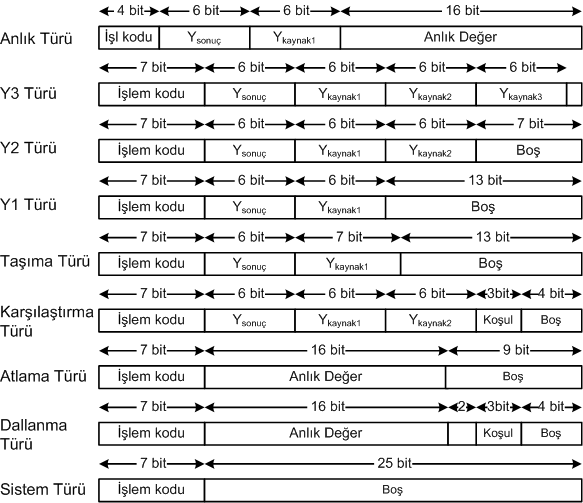
\includegraphics[width=0.9\textwidth]{gorsel/instructionTypes.png}
\shorthandoff{=}
\caption{Tosun Buyruk Türleri}
\label{image:instructionTypes}
\end{figure}

Anlık türü buyruklar bir kaynak yazmacı, bir hedef yazmacı ve bir anlık değer içerir. Dolayısıyla işlem kodu için yalnızca 4 bitlik boş yer kalır. 4 bit, işlem koduna yeterli olmadığı için, olası tasarım çözümleri anlık değerin daraltılması veya buyruk genişliğinin artırılmasıdır. Buyruk genişliğinin değiştirilmesi durumunda bellek yönetimi, buyruk çekme ve kod çözme donanımları karmaşıklaşırken anlık değerin daraltılması durumunda ilave buyruklar gerekeceği gibi, programcının da tasarımı karmaşıklaşmaktadır. Bu probleme özel bir çözüm olarak anlık türü buyrukların 4 bit işlem koduna sahip olmasına karar verilmiştir. Anlık buyruklarda işlem koduna 4 bit ayrılmış olması, işlem kodunun kalan alt bitlerinin x ile doldurulması anlamına gelir. Toplamda 9 adet anlık türü buyruk bulunmaktadır. Dolayısıyla üst 4 biti [0,9] aralığında olan işlem kodları anlık türünde, [10,15] aralığında olan işlem kodları ise diğer türlerdedir. Buyruk kümesinde anlık türü olmayan, 46 adet buyruk vardır. Üst 4 bit için kullanılmayan 6 farklı değer olduğundan alt bitler için 8 farklı değer, dolayısıyla 3 bit gereklidir. \par

Anlık türü buyruklardan kaynaklı bu değişiklik ile Tosun buyrukları 7 bit işlem kodu ile ifade edilir, 0000000 - 1001111 aralığındaki işlem kodları anlık türü buyruklara karşılık gelir, anlık türü buyruklarda alt 3 bit önemsiz olarak kabul edildiğinden yalnızca üst 4 bit buyruk içinde yer alır. Örneğin 0000xxx işlem kodu addi buyruğuna karşılık gelir. Dolayısıyla alt 3 bit buyruğun bit dizisi içinde yer almaz ve gelen herhangi bir buyruk için üst 4 bit 0000 ise buyruğun addi olduğu anlaşılır. Tüm buyruk türlerinin bit yapısı Şekil \ref{image:instructionTypes}'ta sunulmuştur. \par



\section{Hesaplama Modülleri}
Buyruk listesinde her bir buyruk için mimariye eklenmesi gereken hesaplama modülleri irdelenmiş, her bir buyruk için verimin yüksek tutulması adına ilgili optimize edilmiş Xilinx IPCore kullanımına öncelik verilmiştir.\par
\begin{itemize}
\item add, addi, sub, subi, abs, chs buyruklarının hesaplamaları tamsayı toplayıcı ipcore kullanılarak yapılır. Bu işlem birimi hem toplama hem çıkarma işlemini gerçeklemektedir.
\item mul ve muli buyrukları integer çarpma IPCore kullanılarak gerçeklenir.
\item and, andi, or, ori, not, xor, xori, brv ve bfr buyrukları mantıksal bit işlemleri yaparlar. Bu buyrukların her biri için ayrı bir işlem modülü kullanılır.
\item min, max ve com buyrukları için iki sayının karşılaştırılması gerekmektedir. Bu üç buyruğun bir karşılaştırıcı modülünü kullanır. Com buyruğu işlem neticesinde büyük, küçük ve eşit bayraklarının değerini değiştirirken min ve max işlemleri sayılardan küçük olanı veya büyük olanı sonuç yazmacına yazar. 
\item div, divi ve mod buyrukları bölme işlemi için hazırlanmış ipcore kullanırlar.  
\item shl, shr, shra buyrukları kaydırıcı modül kullanılarak gerçeklenirler.
\item f2int ve int2f buyrukları float ve integer veri tipleri arasında dönüşüm sağlar. Her ikisi için de hazır IPCore gerçeklenir.
\item fadd ve fsub buyrukları için float toplayıcı IPCore kullanılarak gerçeklenir.
\item fabs ve fchs buyrukları IEEE754 standardında işaret bitinin değiştirilmesi ile sağlanabilir. Bu iki buyruk için tek bir bit operasyon modülü gerçeklenir.
\item fcom, fmin ve fmax işlemleri floating point bir karşılaştırıcı IPCore kullanırlar.
\item fdiv ve fmod işlemleri floating point bir bölücü IPCore kullanılarak gerçeklenir.
\item fexp  $e^{x}$ hesabı yapan IPCore kullanılarak gerçeklenir.
\item ffma ve ffms işlemleri floating point fused multiply add IPCore kullanılarak gerçeklenir.
\item fln buyruğu floating point doğal logaritma IPCore kullanılarak gerçeklenir.
\item fmul buyruğu floating point çarpma IPCore kullanılarak gerçeklenir.
\item fsqrt buyruğu floating point karekök IPCore kullanılarak gerçeklenir.
\item fsin ve fcos buyrukları trigonometri IPCore kullanılarak gerçeklenir.
\end{itemize}

\section{Boru Hattı Mimarisi}
Buyruk kümesinde bulunan her buyruğun çalıştırılması sırasında geçmesi gereken sabit adımlar vardır. Öncelikle bir buyruk bellekten çekildikten sonra işlem kodu okunmalı ve uygun şekilde bitler ayrılarak buyruk içinde gelen yazmaç numaraları, anlık değerler vb. ayrıştırılmalıdır. Sonrasında ilgili yazmaçlarda tutulan değerler okunmalı, buyruk ile ilgili işlem seçilip okunan değerler üzerine uygulanmalı ve son olarak sonuç yazmacına sonuç yazılmalıdır. Bu adımlar arasına flip floplar eklenerek bir buyruğun adımları ardışık saat vuruşlarında takip etmesi sağlanabilir. Böylece bir buyruğun geçtiği adımdaki donanımlar boşa çıkar ve söz konusu buyruk tüm işlemleri tamamlamadan yeni bir buyruk aynı donanımları kullanarak hesaplamaya girebilir. Boru hattı tasarımında kaynakların etkin kullanımı son derece önemlidir. Eğer programın genelinde tüm boru hattı aşamaları aynı anda doldurulamıyorsa boru hattı kullanmanın avantajı yoktur. Öte yandan boru hattı aşamaları etkin bir şekilde doldurulabilirse buyruklar birbirinin çalışma sürelerini gizlerler ve her saat vuruşunda yeni bir sonuç üretilmiş olur.   \par

Boru hattı aşamalarının tam doldurulması konusunda güncel problemlerin başında veri bağımlılıkları gelir. Eğer n. buyruğun kullanacağı bir veri m. buyruk tarafından hesaplanıyorsa, m. buyruk sonucu yazmaç öbeğine yazmadan n. buyruk yazmaç değerlerini okuyamaz. Veri bağımlılığı önlenemeyen bir problemdir. Bunun yerine literatürde veri bağımlılığı olmayan buyrukların, bekleyen buyrukların önüne alınması yöntemiyle çözülmektedir. Bu yaklaşıma "Out of order execution" ismi verilir. \cite{superscalar600mhz} \cite{superscalarpatent}\par

Sırasız çalıştırma yöntemi beraberinde yazmaçların analizi, veri bağımlılıklarının çözülmesi, yazmaçların donanım seviyesinde yeniden adlandırılması, yazmaç sayıları ile ilgili bir sanallaştırma katmanı tanımlanması gibi donanımsal karmaşıklıkları da beraberinde getirmektedir. Oysa ki aynı anda çok fazla threadin koşturulacağı bir işlemcide, boru hattının etkin kullanımı için daha sade bir çözüm olarak aralıklı işlem modeli kendini gösterir. \cite{interleavedMultithreading} 

Aralıklı İşlem Modeline göre çalışan işlemciler her bir buyruğun çalıştırılmasında sonra farklı bir thread’e geçiş yaparak çalışırlar. Çok sayıda birbirinden bağımsız işlemi bir arada yürütmeye çalışan işlemciler için Aralıklı İşlem tercih edilen bir yöntemdir \cite{Controldatacorp} \cite{TeraMTA}. Bu şekilde çalışan işlemciler her bir thread için ayrı yazmaç öbeği ve program sayacı tutar. Herhangi bir thread’den boruhattına buyruk ataması yapıldığı zaman, farklı bir thread seçilerek bir sonraki buyruk o thread’in program sayacının gösterdiği yerden çekilir.\par

Aralıklı İşlem Modelinde veri bağımlılığı oluşmadığı için boruhattının etkin kullanımı sağlanmış olur. Farklı thread’ler arasında, yazmaç bazında, veri paylaşımı olmadığı için farklı thread’lerden buyrukların boruhattına alınması veri bağımlılığı sorunlarına yol açmaz. Böylece çok sayıda çevrim gerektiren buyruklar, farklı thread’lerden gelen buyrukların çalıştırılmasıyla gizlenmiş olur. Örnek vermek gerekirse, Tosun mimarisinde sin/cos işlemleri 28 saat vuruşunda tamamlanmaktadır. Tek bir thread üzerinden çalışan bir sistem düşünülürse bu sin/cos buyruğundan sonra gelen ve bunun sonucunu kullanan buyruk sin/cos’un tamamlanmasını beklemek zorunda kalır. Bu uzun süre içerisinde de boru hattının büyük bir bölümü boşta bekler. Aralıklı İşlem Modelinde ise aralarında veri bağımlılığı olma ihtimali olmadığı için farklı thread’lerden gelen buyruklar boruhattının içine alınabilir. Böylece sin/cos veya diğer çok sayıda saat vuruşunda sonuç veren işlemler için geçen süre başka buyrukların çalıştırılmasıyla gizlenmiş olur.\par

Aralıklı işlem modelinin bir sonucu olarak farklı threadler arasında hızlı bir şekilde "context switch" yapmak gerekmektedir. Yani bir thread çalışırken bir anda farklı bir threade geçilebilmesi gerekmektedir. Klasik işlemcilerde tüm yazmaç verilerinin belleğe kaydedilmesi ve diğer threade ait verilerin bellekten kopyalanmasıanlamına gelen context switch oldukça pahalı bir işlemdir. Oysa ki aralıklı işlem modelinden faydalanabilmek için 1 saat çevriminde context switch yapılması gerekmektedir. Bu hızda bir context switch ancak farklı threadlere ait yazmaçların da yazmaç öbeğinin bir kısmında saklanması ile mümkün olur. Tosun mimarisinde bu işlemin nasıl yapıldığı "Yazmaç Öbeği" başlığı altında anlatılacaktır.\par

Aralıklı işlem modeli ile çalışan Tosun boru hattı mimarisinin aşamaları şekil \ref{image:pipelineStages}'de gösterilmiştir.

\begin{figure}[h]
\centering
\shorthandoff{=}
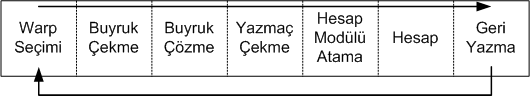
\includegraphics[width=0.9\textwidth]{gorsel/pipelineStages.png}
\shorthandoff{=}
\caption{Tosun Boru Hattı Mimarisi}
\label{image:pipelineStages}
\end{figure}

\subsection{Warp Seçimi}
Warp NVidia tarafından literatüre kazandırılmış bir terimdir. Threadlerin bir araya toplanması ile oluşan thread grubuna warp ismi verilmiştir. Thread sözlükte ipliğe karşılık gelirken warp da dokumacılıkta kullanılan çözgü anlamını taşımaktadır. N adet threade sahip bir uygulamanın M adet SIMD Lane kapasitesi bulunan bir işlemcide çalıştırılması senaryosunda 3 farklı ihtimal vardır. N = M ise her bir SIMD lane üzerinde bir thread koşturulur. N < M ise bazı SIMD lane'ler boş kalır ve bunların sonuçları değerlendirilmez. En sık rastlanan durum olan N > M olması durumunda ise N adet thread M adet kapasiteli alt gruplara bölünür ve bir seferde M adet thread çalıştırılır. Arkasından ikinci ve üçüncü M adet thread barındıran gruplar çalıştırılır. Burada her M adet thread'den oluşan gruba warp ismi verilir. Dolayısıyla warp kapasitesi donanımda tanımlı SIMD lane sayısına bağlı iken warp sayısı uygulamadaki toplam thread sayısının warp büyüklüğüne bölümü ile hesaplanır. Threadlerin warplara ayrılma işlemi derleyici tarafından yapılır.\par 
Aralıklı işlem modelinin bir uygulaması olarak, bir SIMD lane'e her saat vuruşunda farklı bir warp'a ait bir thread atanır. Hangi warp'un seçileceği boru hattının "Warp Seçimi" aşamasında belirlenir. Bu seçim Round-Robin politikasına göre gerçekleştirilir. Her warp için durum bitleri tutulur. Bu bitler warp'un "yürütme için uygun", "çalışıyor", "tamamlandı" gibi durumlarını gösterir. Uygun olan warp'lardan biri seçilir ve bu warp'un numarası boru hattının bir sonraki aşamasına aktarılır. Seçilen warp, boru hattını tamamlamadan bir daha seçilememesi için durum bitleri değiştirilerek işaretlenir. Aynı warp'un bir kez daha boru hattına alınması thread'lerin bir sonraki buyruklarının işlenmesi anlamına gelir. Bir warp boru hattını tamamlamadan ikinci kez boru hattına alınmadığında ikinci buyruk da boru hattına girmemiş olacağından herhangi bir veri bağımlılığı kontrolüne gerek kalmaz.\par
\subsection{Buyruk Çekme}
Buyruk çekme aşamasında bir önceki aşamadan gelen warp id'nin sıradaki buyruğu bellekten çekilir. Program buyrukları harici RAM’de tutulur. Buyruklara erişim program akışı sebebiyle genel olarak sıralı ve aralıklı işlem modeline göre tekrarlı olduğu için RAM’den gelen buyrukları bir süre Buyruk Önbelleği yapısında tutmak bu aşamayı oldukça hızlandıran bir optimizasyondur. Buyruğun çekilmesi ile bu aşama tamamlanır ve buyruk bir sonraki aşamaya geçirilir.
\subsection{Buyruk Çözme}
Bu aşamada buyruk çözümlenerek hangi işlem biriminin kullanılacağı, hangi yazmaçların okunup, hangilerine yazılacağı belirlenir. Tüm buyrukların 32 bit olması, işlem kodu genişliklerinin buyruklar arasında fazla farklılık göstermemesi ve neredeyse tüm buyrukların aynı yazmaçlara erişim yapabilmesinden dolayı, boru hattının bu aşaması sade bir yapıdadır.
\subsection{Yazmaç Çekme}
Burada çalıştırılmak üzere olan buyruğun işlem sırasında kullanacağı verilen yazmaç öbeğinden alınır. Her bir SIMD lane üzerinde her bir warp için ayrı bir Yazmaç Öbeği vardır ve bunlardan kullanılacak veriler aynı anda çekilir. İki adet kaynak yazmacı bulunan buyruklarda ve 16 çekirdekli bir adada toplam 32(16*2) adet 32-bitlik veri ortalama 1 çevrimde okunur.
\subsection{Hesap Modülü Atama}
Boru hattının bu aşaması hesaplamanın başlatıldığı yerdir. Bu aşamaya gelen bir buyruğun tüm verileri hesaplamaya hazır bir halde beklemektedir. Bu aşamada işlem koduna bakılarak buyruk gerekli hesaplama donanımına gönderilir.
\subsection{Hesap}
Hesaplamanın yapıldığı aşamadır. Burada birçok işlem birimi yer alır. Bunlardan, sık kullanılan ve daha az alan kaplayan işlem birimleri SIMD lane adetindedir. Bu şekilde, bu işlem birimleri gelen tüm verileri aynı anda işleme sokabilecek durumdadır. Daha nadir erişilen trigonometrik işlemler ve logaritma gibi hesaplardan sorumlu işlem birimleri ise daha az sayıda bulunabilir. Az sayıda bulunan işlem birimlerinin kendi boru hattı mevcuttur. Örneğin SIMD lane sayısının yarısı adetinde olan bir hesaplama modülü ilk çevrimde gelen sayıların yarısını işleme alır, ikinci çevrimde ise diğer yarısını işleme alır. Böylece tüm sayılar boru hattında peşi sıra ilerlemiş olurlar. Örneğin 28 çevrim süren bir sinus işlemi için SIMD lane sayısının çeyreği kadar sinus hesaplama birimi yerleştirilmişse, tüm sayıların sinus sonuçlarının hesaplanması 28 + 3 = 31 çevrim sürer. Alan kullanımı ve performans optimizasyonu için esneklik sağlayan bu yapıda ilave 3 çevrim kabul edilerek alandan kazanılabilir ya da hesap modülü sayısı artırılarak performans artışı sağlanabilir. Hesap aşamasının sonunda bir sonuç buffer'ı bulunmaktadır. Hesap modüllerinin boru hattından çıkan sonuçlar önce bu buffer'lara yazılır ve yazılmak için kendi sıralarının gelmesini beklerler. 
\subsection{Geri Yazma}
Geri yazma aşaması sonuçların yazmaç öbeklerine yazıldığı aşamadır. Geri yazma aşamasının kontrolcüsü sürekli olarak hesap modüllerinin çıkışlarındaki sonuç buffer'larını kontrol eder ve sırasıyla sonuçları ilgili yazmaçlara yazar.

\section{Veri Yolu Mimarisi }
Önceki bölümlerde Tosun mimarisinin buyruk kümesi, hesaplama donanımları ve boru hattı aşamaları belirlenmiştir. Parçaların birleştirilmesi ile veri yolu mimarisi oluşacaktır. Tasarım gereksinimleri arasında belirtilen ölçkelenebilirlik özelliğinden dolayı tüm kodlama parametrik olarak yapılmıştır. Mimarinin üzerine inşa edildiği temel parametrelerden biri de SIMD lane sayısıdır. SIMD lane sayısındaki artış, veri yolu genişliklerinin, karşılaştırıcı, kod çözücü ve kodlayıcı gibi donanımların katlanarak artmasına sebep olmaktadır. Bu etki hem alan kullanımında hem de sinyal gecikmelerinde artışa neden olur. Neticede performans kaygısı ile paralelliğin artması için SIMD lane sayısının artırılması ile alan kullanımı büyümekte, gecikmeler artmakta ve hem güç tüketimi artmakta hem saat sıklığı azalmaktadır. Dahası FPGA içi routing işlemi de SIMD lane sayısının artması ile zorlaşmakta ve imkansız hale gelebilmektedir. Bu etki, kaçınılmaz olmakla beraber hiyerarşik tasarım kullanılarak azaltılabilir.\par 

Tosun mimarisi routing ve timing ile ilgili kısıtları zorlayabilmek adına hiyerarşik bir yapıda tasarlanmıştır. Doğrudan N adet SIMD lane gerçeklenmesi yerine küçük gruplar halinde, $N=N_{1}xN_{2}$ olacak şekilde $N_{1}$ adet ada ve her adanın içinde $N_{2}$ adet SIMD lane olacak şekilde gerçeklenmiştir. Hiyerarşinin üst seviyesinde, ölçeklenebilirliği olmayan PCI-e ve Ana bellek arayüzü gerçeklenmiş ve AXI bus yapısı ile N adet ada ismi verilen donanıma bağlanmıştır. Tosun üst seviye mimari çizimi Şekil \ref{image:genelMimari}’da sunulmuştur. Mimarinin büyük tek bir ada yerine çok sayıda daha küçük adalardan oluşmasının iki sebebi  vardır. \par
\begin{figure}[h]
\centering
\shorthandoff{=}
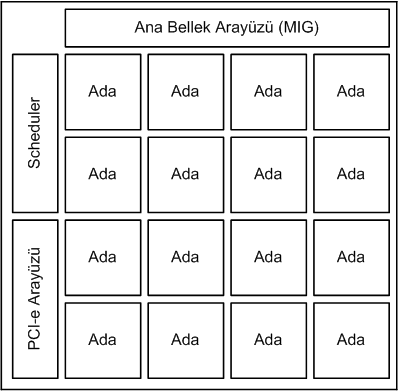
\includegraphics[width=0.5\textwidth]{gorsel/genelMimari.png}
\shorthandoff{=}
\caption{Tosun Üst Seviye Mimarisi}
\label{image:genelMimari}
\end{figure}
Her bir ada içindeki threadlerin veri paylaşabilmesi için ada içine yerleştirilen paylaşımlı belleğe erişimi olan çekirdek sayısı ile bu bellekte yaşanan gecikme doğrudan ilişkilidir. Paylaşımlı bellek açısından bakıldığında istemci sayısının artması istek paketlerinin beklediği kuyrukta uzamaya sebep olmaktadır. Bu durum sınav zamanında kütüphaneden kitap almak isteye öğrenciler analojisiyle açıklanabilir. Her bir öğrenci bir istek paketi, ulaşmak istedikleri kitaplar da paylaşımlı bellekte tutulan veriler olsun. Kütüphanede kitap ödünç alımıyla ilgilenen personel sayısını sabit olarak 2 kabul edelim. Kitap sayısı sonsuz bile olsa, N adet öğrencinin bu iki personel üzerinden kitaplara erişim imkanı varken, öğrenci sayısının artması ile bir öğrencinin ortalama kitaba ulaşma süresi doğru orantılı olarak artacaktır. Artışı engellemek için yapılabilecek iki seçenekten birincisi öğrenci sayısını sınırlamak, ikincisi ise personel sayısını artırmaktır. Bu analojide personel sayısı FPGA üzerinde gerçeklenen Block RAM'lerin port sayısını ifade eder. Block RAM'lerin port sayısı 2'den fazla olamadığından istemci sayısını azaltmak tek çözümdür. Bu bağlamda tasarımı adalara ayırmak, kütüphaneyi parçalamaya ve kütüphane başına düşen öğrenci sayısını azaltmaya benzer. Dolayısıyla çok sayıda çekirdeği küçük gruplar halinde ayırarak her gruba bir paylaşımlı bellek tahsis etmek bellek işlemlerinin performansını artıracaktır. \par
Diğer bir sebep ise yukarıda bahsedilen, FPGA gerçeklemesi sırasında oluşabilecek timing ve routing problemleridir. Yapılan bir tasarım FPGA üzerinde gerçeklenirken herhangi bir kısıt tanımlanmamışsa birbirine yakın olması beklenen bazı donanım parçaları yonga üzerinde uzak yerlere denk gelebilir. Ölçeklenebilir tasarımlarda bu problem sıklıkla kaynakların verimsiz kullanımına ve tellerin uzaması ile kritik yollardaki gecikmelerin artmasına dolayısıyla saat frekansının düşmesine ve nihayetinde performans düşüşüne sebep olabilir. Bu problemlerden kaçınmak için sıklıkla hiyerarşik tasarımlar gündemde tutulur. Tosun tasarımının homojen adalardan oluşması sentez aracına hangi donanımların yakın olması gerektiği konusunda daha çok fikir vermekte ve bu konudaki potansiyel problemlerin indirgenmesine olanak sağlamaktadır.\par 
Tasarımın adalara ayrılması ile donanım seviyesinde bir soyutlama sağlanmıştır. Bu soyutlama, Tosun üzerinde o anda koşan tüm threadlerin aynı anda aynı buyruklarının koşması zorunluluğunu ortadan kaldırır. SIMD mimarinin bir özelliği olarak herhangi bir t anında ada içerisinde çalışan tüm threadlerin aynı buyrukları koşmakta, bütün threadler için o buyruk tamamlanmadan diğer buyruğa geçilmemektedir. Öte yandan aynı anda farklı adalarda farklı buyruklar çalışıyor olabilir. Bu sayede ana bellek erişimi farklı adalar için farklı zamanlarda gerçekleşebilir; böyle bir durumda beklemeler azalır. Farklı adaların farklı zamanlarda bellek erişimi istemesi ise ilk bellek erişiminden sonra kaçınılmazdır.  

\subsection{Ada İçi Veri Yolu Mimarisi}

Yukarıda anlatılan buyrukların koşturulduğu ve boru hattının uygulandığı mimari ada içi mimaridir. Her adanın içinde N adet SIMD lane var ise N adet yazmaç öbeği bulunmaktadır. Alan tüketimi az olan ve hedef uygulamalarda sıkça kullanılan hesaplama birimlerinden de N adet bulunmaktadır. Diğer buyruklara oranla daha az sıklıkta kullanılan ve alan tüketimi yüksek olan hesaplama birimlerinden ise $N/2^{k}, k\in[1,log_{2}N]$ adet kullanılır. Uzun süren hesaplama modüllerinin içinde de boru hattı bulunmaktadır. Bu sayede modül sayısının $N/2^{k}$ olduğu durumda sadece k çevrim maliyeti olur.\par
\begin{figure}[h]
\centering
\shorthandoff{=}
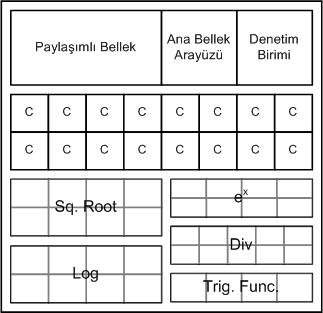
\includegraphics[width=0.5\textwidth]{gorsel/adaMimarisiEski.png}
\shorthandoff{=}
\caption{Tosun Ada Mimarisi (Kavramsal)}
\label{image:adaMimarisiEski}
\end{figure}

\begin{figure}[h]
\centering
\shorthandoff{=}
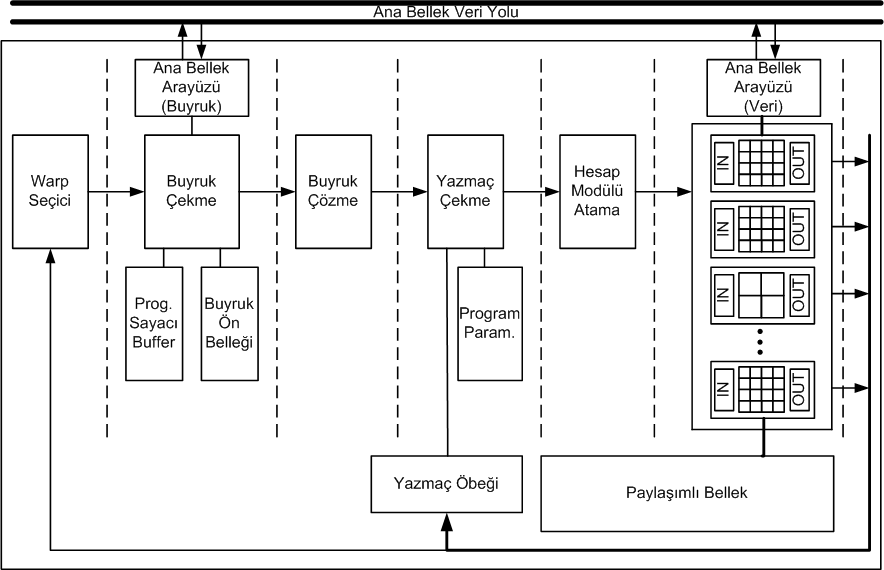
\includegraphics[width=0.9\textwidth]{gorsel/adaMimarisi.png}
\shorthandoff{=}
\caption{Tosun Ada Mimarisi (Boru Hattı)}
\label{image:adaMimarisi}
\end{figure}

Ada içi mimarinin kavramsal gösterimi şekil \ref{image:adaMimarisiEski}'de boru hattı ile gösterimi şekil \ref{image:adaMimarisi}'de sunulmuştur. Her bir buyruk boru hattı üzerinde ilerleyerek işlenir. Boru hattının etkin kullanımı için daha önce belirtilen aralıklı işlem modeli kullanılır ve her saat vuruşunda farklı bir warptan işlem alınır. \par
Bir adada koşturulan thread sayısı adanın SIMD lane sayısı kadardır. Aralıklı işlem modelinin uygulanabilmesi için adada koşturulan warplara ait yazmaç bilgilerinin tamamının yazmaç öbeğinde saklanması gerekir. Dolayısıyla adada koşturulan warp sayısı yazmaç öbeğinin büyüklüğüne bağlıdır.\par

\subsubsection{Yazmaç Öbeği Tasarımı}
NVidia benchmarkları üzerinde yapılan analizlerde thread başına 64 yazmacın yeterli olacağı tespit edilmiş ve buyruk kümesi de 64 yazmaca göre tasarlanmıştır. Aralıklı işlem modelinin uygulanabilmesi için her saat vuruşunda yeni bir warp'un boru hattına alınması gerekmektedir. Ana boru hattı 7 aşamadan oluşmakta, hesaplama işlemleri ise 28 vuruşa kadar çıkmaktadır. Boru hattını doldurabilecek sayıda olması açısından ada içindeki warp sayısının minimum 32 olması gerekmektedir. Dolayısıyla her bir SIMD lane için yazmaç öbeği büyüklüğü 64 yazmaç x 32 warp x 32bit = 64kbit kapasiteli olmalıdır. 32kbit büyüklüğünde 2 block ram primitive kullanılarak yazmaç öbeği tasarlanabilir.\par
\begin{figure}[h]
\centering
\shorthandoff{=}
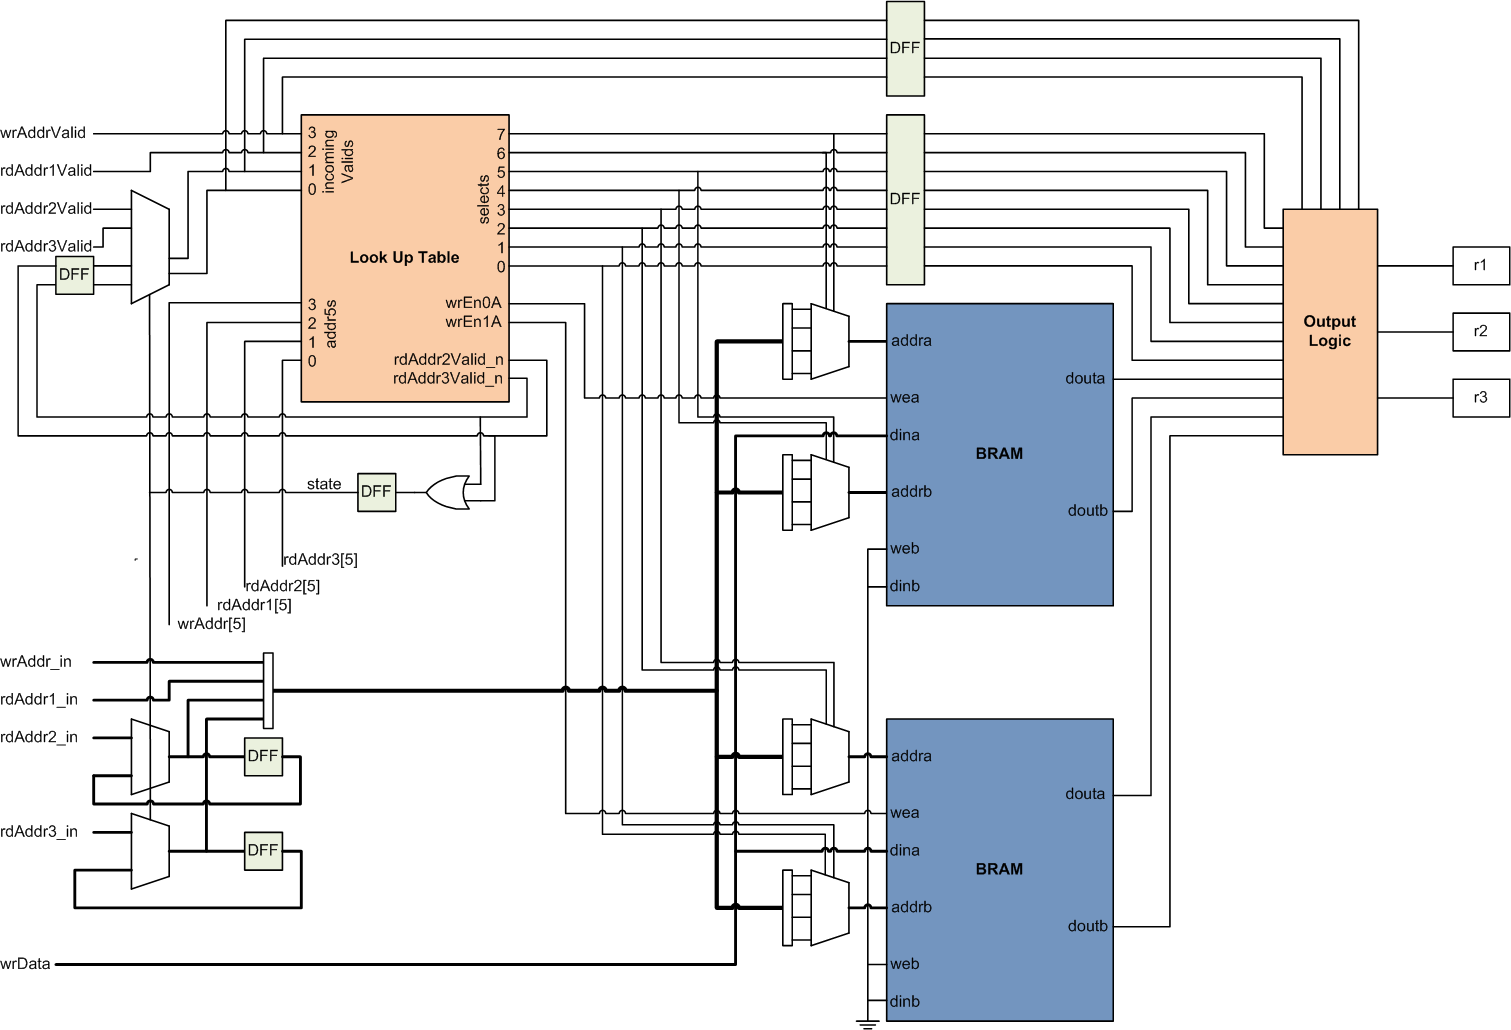
\includegraphics[width=\textwidth]{gorsel/registerFile.png}
\shorthandoff{=}
\caption{Tosun Yazmaç Öbeği}
\label{image:registerFile}
\end{figure}
Şekil \ref{image:registerFile}’de gösterilen yazmaç öbeği 2 adet true dual port BRAM kullanmaktadır. Dolayısıyla toplam 4 adet fiziksel port bulunur. Buyruk kümesinde var olan buyruklara göre aynı anda en fazla 3 okuma ve 1 yazma operasyonu (4 portlu) gelmektedir. 4 port üzerinden gelen isteklerin BRAM’lere bağlı 4 porta aktarılabilmesi için adreslerin 2’şerli gruplandığında farklı BRAM’leri göstermesi gerekir. Bu durumun her zaman olacağı garanti edilemeyeceğinden portlara bir öncelik ataması yapılmış (WR > RD1 > RD2 > RD3) ve önceliği düşük olan 2 portun sonraki çevrim(ler)de işlenebilmesi için gerekli hafıza birimleri yerleştirilmiştir. Burada en kötü durum tüm portların aynı BRAM’e ait adresleri göstermesidir.  Böyle bir durum oluştuğunda WR ve RD1 portunun istekleri aynı çevrimde işlenirken RD2 ve RD3 portları sonraki çevrimde işlenmek üzere bekletilir. Eğer sonraki çevrimde yeni bir WR operasyonu gelirse WR ve RD2 işlenir, RD3 bekletilir. Nihayetinde en kötü durumda 3. Çevrimde RD3’ün de okunması ile okuma işlemi tamamlanmış olur. Özetle Şekil \ref{image:registerFile}’de gösterilen tasarıma sahip bir yazmaç öbeği kümesinde bulunan yazmaç öbeklerinde en kötü durum için yazma işlemi 1 çevrimde okuma işlemi 3 çevrimde tamamlanmaktadır. Bu gecikmeler BRAM kısıtlarından kaynaklanmaktadır. \par
Yazmaç öbeği okuma işlemlerinin en kötü durumdaki cevap süresini kısaltmak mümkün olmasa da en kötü durumun oluşma ihtimalini azaltmak mümkündür. Bir iyileştirme olarak her bir thread’e ait 64 adet yazmaçtan oluşan yazmaç öbeği, 32 yazmaçlık 2’şer gruba bölünerek tüm thread’lere ait yazmaç öbeklerinin ilk yarıları ilk BRAM’de, ikinci yarıları ise ikinci BRAM’de saklanır. Bu saklama şekli sabit tutularak derleyicinin yazmaçları seçerken bu ayrımı göz önünde bulundurulması sağlanmakta ve en kötü durumun oluşma ihtimali en aza indirgenmektedir. \par
Yazmaç Öbeği Kümesi 11 bit ile adreslenir. Soldaki 5 bit warp numarasını, sağdaki 6 bit ise yazmaç numarasını belirtir. Bu şekilde farklı bir warp'a geçiş yapılacağı zaman sadece bu adresin 5 bitlik prefix’inin değiştirilmesi yeterli olur. Dolayısıyla hiç saat vuruşu kaybetmeden context switch yapılabilir.
\subsubsection{Hesaplama Modülleri}
Tüm işlemler için hesaplama modüllerinin yapısı aynıdır. Giriş ve çıkışlardan da sadece “sayılar” girişleri içerideki birime göre değişken olabilir, diğer tüm giriş ve çıkışlar ise standarttır. Örneğin; toplama birimi için 2 adet 32-bitlik giriş varken, multiply-add işlemi için 3 adet sayı gerekir. Şekil \ref{image:executionUnitIO}'de “N” hesaplamada kullanılan eleman sayısını göstermektedir.\par
\begin{figure}
\centering
\shorthandoff{=}
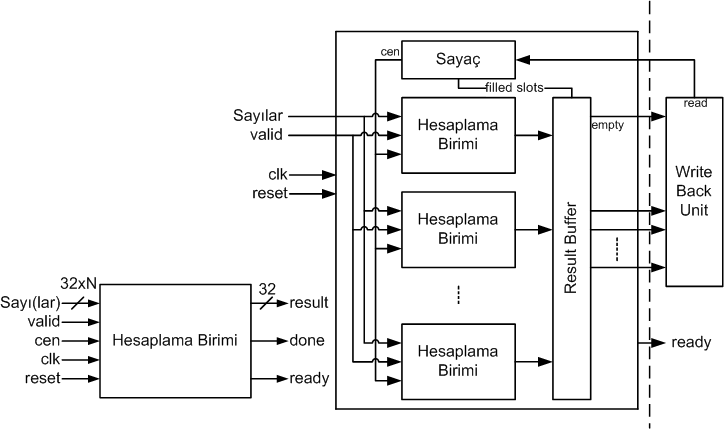
\includegraphics[width=0.9\textwidth]{gorsel/executionUnitIO.png}
\shorthandoff{=}
\caption{Hesaplama Modülleri}
\label{image:executionUnitIO}
\end{figure}
Hesaplama modülleri \ref{image:executionUnitIO}'de sağ tarafta gösterildiği gibi Hesaplama Grubu’nu oluşturur. Burada en fazla çekirdek sayısı kadar olmak üzere değişken sayıda işlem birimi yer alabilir. Grup içerisindeki işlem birimlerinin paylaştığı  Sonuç Buffer'ı vardır. Sonuç Buffer'ı yine Hesaplama Grubu içerisinde yer alan “sayaç” ile birlikte bir FIFO yapısı gibi davranır. Hesaplama Birimlerinden çıkan sonuçlar Sonuç Buffer’ına yazılır ve "Geri-Yazma" biriminin bu verileri okuyup yazmaç öbeğine yazması beklenir. Geri yazma birimi round robin algoritmasını kullanarak hazır olan verileri sıradan yazmaç öbeğine yazar.

\subsubsection{Paylaşımlı Bellek}
Threadlerin yazmaçları kendilerine özel olup dışarıdan bir modülün erişimi yoktur. Oysa ki paralel hesaplamalarda bir threadin ürettiği bir sonuç başka bir thread tarafından kullanılabilir. Threadler arası veri paylaşımı için iki seçenek vardır. Bir seçenek ana bellek üzerinden veri paylaşımı yapılması iken diğeri paylaşımlı bellek eklenmesidir. Ana bellek hem yonga dışında olduğundan hem de veri yolu genişliğinin sınırlı olmasından dolayı yavaş olacaktır.\par
FPGA üstünde paylaşımlı bellek gerçeklemesi ancak Block RAM kullanımı ile mümkündür. Donanımda tanımlı Block RAM Primitive'ler 32KB büyüklüğünde olup 2 portu desteklemektedir. Paylaşımlı bellek kapasitesinin artırılması birden fazla Block RAM Primitive üzerine adres uzayı taksim edilir.\par
Her bir çekirdeğin paylaşımlı belleğe erişiminin bulunması gerekmektedir. Bunun için çekirdek sayısı adetinde porta sahip bir paylaşımlı bellek Block RAM Primitive'ler kullanılarak Şekil \ref{image:sharedMemory}'de gösterildiği şekilde tasarlanmıştır.
\begin{figure}[ht]
\centering
\shorthandoff{=}
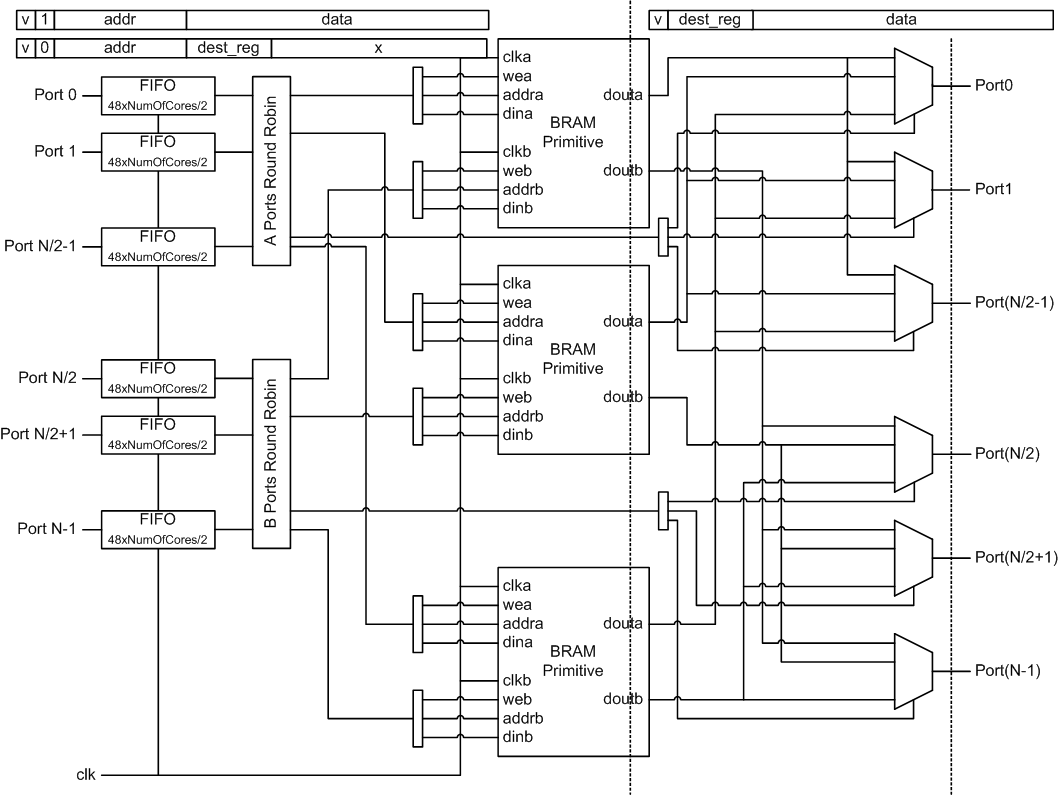
\includegraphics[width=0.9\textwidth]{gorsel/sharedMemory.png}
\shorthandoff{=}
\caption{Tosun Paylaşımlı Belllek Mimarisi}
\label{image:sharedMemory}
\end{figure}

Paylaşımlı belleğin girişindeki her bir port bir SIMD lane'e bağlıdır. Paylaşımlı belleğin içinde N adet 32kB Block RAM Primitive şekil \ref{image:sharedMemory}'de gösterildiği gibi giriş portlarına öncelik atayıcı donanımlar üzerinden bağlıdır. Her block ram portu için bir öncelik atayıcı bulunmakta ve o block ram portunun hangi SIMD lane portu ile bağlanacağına karar vermektedir. Herhangi SIMD lane üzerinde paylaşımlı belleğe yazma veya okuma amaçlı erişmek isteyen bir buyruk olursa, o SIMD lane'e bağlı port üzerinden ilgili öncelik atayıcıya istek gelir. Her saat vuruşunda öncelik atayıcılar kendilerine gelen istekler üzerinden Round Robin algoritması ile bir seçim yapar. Seçilen paket block ram'e iletilirken, seçilmeyen paketler sırada tutulur. Bunun için her SIMD lane portunun girişinde bir FIFO tampon bellek bulunmaktadır. Her block ram primitive 2 adet porta sahip olduğu için SIMD lane portları ikiye bölünür. Yarısı block ram primitive'lerin A portlarına bağlanırken diğer yarısı B portlarına bağlanır.\par

Paylaşımlı bellek mimarisi için en kötü durum tüm SIMD lane portlarından aynı block RAM primitive için istek paketleri gelmesidir. Bu durumda SIMD lane sayısının yarısı büyüklüğünde kuyruk oluşur ve işlemler buna göre gecikmeli gerçekleşir. En kötü durum ihtimalini ortadan kaldırmak mümkün değildir fakat ihtimali düşürmek adına adres uzayının block ram'lere dağıtım yönteminde iyileştirme yapılabilir. \par

Tosun paylaşımlı bellek mimarisinde kullanılan verilerin tamamı 32 bit genişliğinde, block ram primitiveler ise 32 kbit büyüklüğündedir. Dolayısıyla her block ram primitive 1000 adet adresten oluşur. Paylaşımlı bellek büyüklüğünün 128kbit olması durumunda toplamda8 adet block ram bulunmaktadır Adres uzayı block ramlere patlaştırılırken üst bitler yeerine alt bitlerin kullanılması ile ardışık adresler her zaman farklı block ram primitive'lerini gösterir ve en kötü durum ihtimali azaltılır. 
